\documentclass{article}
\usepackage[utf8]{inputenc}
\usepackage{amsmath}
\usepackage{tcolorbox}
\usepackage[margin=1in]{geometry}
\usepackage{listings}
\usepackage{xcolor}
\usepackage{mathtools}

\definecolor{codegreen}{rgb}{0,0.6,0}
\definecolor{codegray}{rgb}{0.5,0.5,0.5}
\definecolor{codepurple}{rgb}{0.58,0,0.82}
\definecolor{backcolour}{rgb}{0.95,0.95,0.92}

\lstdefinestyle{mystyle}{
    backgroundcolor=\color{backcolour},   
    commentstyle=\color{codegreen},
    keywordstyle=\color{magenta},
    numberstyle=\tiny\color{codegray},
    stringstyle=\color{codepurple},
    basicstyle=\ttfamily\footnotesize,
    breakatwhitespace=false,         
    breaklines=true,                 
    captionpos=b,                    
    keepspaces=true,                 
    numbers=left,                    
    numbersep=5pt,                  
    showspaces=false,                
    showstringspaces=false,
    showtabs=false,                  
    tabsize=2
}

\lstset{style=mystyle}

\usepackage{hyperref}
\hypersetup{
    colorlinks=true,
    linkcolor=blue,
    filecolor=magenta,      
    urlcolor=cyan,
}


\title{Logistic Regression and Gradient Descent \\ Logic and Python tutorial}
\author{Sophie Marchand}
\date{May 2020}

\begin{document}

\maketitle

\section{Shortcut}
\begin{tcolorbox}
The logistic regression is used to solve binary classification problem by modelling the probability \(p\) of belonging to the class \(0\) (or \(1\)) through logarithm transformation and linear combination of input variables such as \((x_{1}, x_{2})\) as follow:
\[ln(\frac{p}{1-p}) = a + b_{1} * x_{1} + b_{2} * x_{2} = -f \xLeftrightarrow[]{} p =\frac{e^{-f}}{1 + e^{-f}}\]

Also, we can estimate the coefficients \((a, b_{1}, b_{2})\) of the logistic regression through the gradient descent with, for example, the cost function \(C\) leading to the coefficient update for \(c \in(a, b_{1}, b_{2})\) with \(\eta\) the learning rate and \(i\) the index of the set of the input and output values \((x_{1}, x_{2}, y)_{i}\):
\[C(i) = \frac{1}{2}(p-y_{i})^{2} \text{  leading to  } c:=c + \eta*\frac{\partial y}{\partial c}*(p-y_{i})*p*(1-p)\]
\end{tcolorbox}

\begin{figure}[h]
\centering
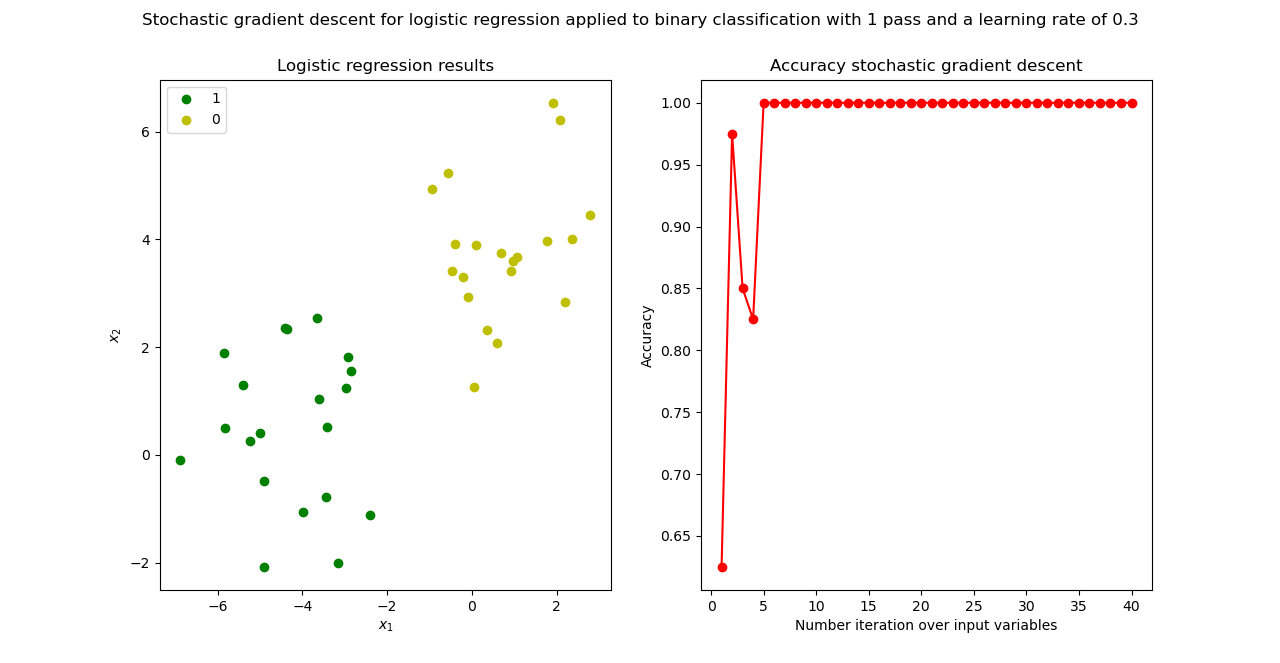
\includegraphics[width=1.05\textwidth]{Figure_LogisticRegressionGradientDescent}
\caption{Output of the tutorial in section \ref{Python tutorial}}
\end{figure}

\section{Logic details}
We present here the intuition behind the logistic regression algorithm and its resolution through stochastic gradient descent. The logistic regression is used to model the odds of belonging to the class \(1\) within a binary classification problem having the classes \(0\) and \(1\). We note \(p\) the probability to belong to the class \(1\), also the odds to belong to this class are defined as:
\begin{equation} \label{1}
    odds_{1} = \frac{p}{1-p}
\end{equation}

The idea of the logistic regression is to represent \(odds_{1}\) as a linear function of the input variables through a logarithmic transformation as presented in equation (\ref{2}). For this demonstration, we have two input variables \((x_{1}, x_{2})\) and the linear coefficients are noted \((a, b_{1}, b_{2})\). 
\begin{equation} \label{2}
    ln(odds_{1}) = ln(\frac{p}{1-p}) = a + b_{1} * x_{1} + b_{2} * x_{2}
\end{equation}

By rearranging the equation (\ref{2}), we obtain the equation (\ref{3}) where \(f = - (a + b_{1} * x_{1} + b_{2} * x_{2})\) is the predicted output variable. 
\begin{equation} \label{3}
    p = \frac{e^{a + b_{1} * x_{1} + b_{2} * x_{2}}}{1 + e^{a + b_{1} * x_{1} + b_{2} * x_{2}}} = \frac{e^{-f}}{1 + e^{-f}}
\end{equation}

We remark that the form of expression (\ref{3}) resembles the logistic function form \(\frac{1}{1+e^{-value}}\) and that is why, this method is called logistic regression. To compute the coefficients \((a, b_{1}, b_{2})\), we use the stochastic gradient descent with the following cost function (\ref{4}) and derivative (\ref{5}). We note \(c\) the considered coefficient among \((a, b_{1}, b_{2})\) and \(y_{i}\) the output variable associated to the input variables \((x_{1,i}, x_{2,i})\).
\begin{equation} \label{4}
    C(i) = \frac{1}{2}(p-y_{i})^{2}
\end{equation}

\begin{multline}\label{5}
    \frac{\partial{C(i)}}{\partial{c}} = (p-y_{i})*\frac{\partial{p}}{\partial{c}} = (p-y_{i})*\frac{\partial{(\frac{e^{-f}}{1 + e^{-f}})}}{\partial{c}} = (p-y_{i})*\frac{e^{-f}}{(1 + e^{-f})^{2}}*-\frac{\partial{y}}{\partial{c}} \\ = -\frac{\partial{y}}{\partial{c}}*(p-y_{i})*\frac{e^{-f}}{1 + e^{-f}}*(1-\frac{e^{-f}}{1 + e^{-f}}) = -\frac{\partial{y}}{\partial{c}}*(p-y_{i})*p*(1-p)
\end{multline}

According to the gradient descent equations (see \href{https://github.com/SophMarch/Tutorials}{GitHub}) and the equation (\ref{5}), we have the following expressions for the coefficients update of the logistic regression with \(\eta\) the learning rate:
\begin{equation}\label{6}
    \begin{cases}
    a := a - \eta\frac{\partial C(i)}{\partial a} = a - \eta*(p-y_{i})*p*(1-p) \\
    b_{1} := b_{1} - \eta\frac{\partial C(i)}{\partial b_{1}} = b_{1} - \eta*(p-y_{i})*p*(1-p)*x_{1,i}\\
    b_{2} := b_{2} - \eta\frac{\partial C(i)}{\partial b_{2}} = b_{2} - \eta*(p-y_{i})*p*(1-p)*x_{2,i}
    \end{cases}
\end{equation}

Finally, using the stochastic gradient descent with 1-to-10 passes based on the equations (\ref{6}), we will obtain the optimal coefficients \((a, b_{1}, b_{2})\) of the logistic regression. In order to identify the class of the input variables \((x_{1}, x_{2})\), we can define a threshold \(p_{th}\) such as:
\begin{equation}
    \begin{cases}
    \text{class } = 1 \text{ for } p\geq p_{th} \\
    \text{class } = 0 \text{ for } p< p_{th}
    \end{cases}
\end{equation}

\newpage
\section{Python tutorial} \label{Python tutorial}
The code source displayed below can be found on \href{https://github.com/SophMarch/Tutorials}{GitHub} under Python\_LogisticRegressionGradientDescent
\lstinputlisting[language=Python]{Python_LogisticRegressionGradientDescent.py}

\end{document}
